

\documentclass[journal]{IEEEtran}


\ifCLASSINFOpdf
  \usepackage[pdftex]{graphicx}

\else

\fi

% Fix the "endthebibliography" macro which produces an error if the bibliography is empty
\makeatletter
\def\endthebibliography{%
  \def\@noitemerr{\@latex@warning{Empty `thebibliography' environment}}%
  \endlist
}
\makeatother





\usepackage{url}
\usepackage{subcaption}
\usepackage{graphicx}

\hyphenation{op-tical net-works semi-conduc-tor}


\begin{document}


\title{Evaluation of the loopback mode of the Adlam Pluto with regard to simple detection and radar tasks }


\author{Fabian Arzberger,
        Jasper Zevering}


\markboth{Report of Telecommunications Lab Project, ~Group 3, ~Vol.~1, No.~\textit{Arzberger/Zevering}, September~2020}%
{Shell \MakeLowercase{\textit{et al.}}: Bare Demo of IEEEtran.cls for IEEE Journals}





% make the title area
\maketitle

% As a general rule, do not put math, special symbols or citations
% in the abstract or keywords.
\begin{abstract}
The loopback mode of the Software Defined Radio (SDR) Adlam Pluto feeds the incoming received RF signals directly to the transmit port, bypassing the internal FPGA structure.
%  Source: https://de.mathworks.com/help/supportpkg/plutoradio/ref/comm.sdrtxpluto-system-object.html#bvn_isv-1_sep_mw_2858fe15-bb5b-4eca-9706-1bca447fac05
In this report, two SDRs are used where one of which is in loopback mode to implement a simple detection of the loopback device.
The implementation of a radar with this setup shows limitations in terms of hardware and software - Python specifically.
Furthermore, the role of the loopback mode regarding these limitations is discussed.
\end{abstract}



\IEEEpeerreviewmaketitle


\section{Introduction}
\label{sec:introduction}

\IEEEPARstart{S}{oftware} Defined Radios (SDRs) open the expensive and complex traditional field of radios for a wide range of users with smaller budget by replacing the unflexible harware-bound components by software. That way, a SDR enables flexible and easy to use changes of the emulated components like mixers, amplifiers, filters, etc. The Adlam Pluto is such a SDR. It is specialized for education and covers a frequency range of 325 MHz to 3.8 GHz with an instantaneous bandwidth up of up to 20 MHz and a 12-bit analog-digital / digital-analog-converter. 
The Pluto has two loopback modes. The digital-TX-to-RX and analog-RX-to-TX mode. The first mode interprets the digital, pure signal which should have theoretically been sent and uses it as the input signal. It is the digital version of connecting the Rx output to the TX input with a cable, but without any distortion or perturbations due to environment and/or hardware. Therefore, this mode has a primary educational use or is used for internal testing. 
The second, analog loopback mode takes the received signal and leads it to the transmitter. Section \ref{sec:behaviourLoopback} shows the exact behavior of the second loopback mode. 
As exemplary practical use, the implementation of detection of a specifically initialized PluoSDR in analog loopback mode is shown. Furthermore, the limitations of it with regard to the realization of distance measurements with the use of this mode are discussed.


\section{Behaviour of Loopback mode}
\label{sec:behaviourLoopback}
The overall idea of the analog RX-to-TX loopback mode is to take the unchanged received signal after processing it with filters, amplifiers etc. and feed that to the input of the transmitter chain.
That means that the signal also goes through all blocks of that transmitter chain.
Therefore, the transmitted signal not only depends on all the blocks of the transmitter chain, as it would also without loopback mode, but the transmitted signal also depends on the received signal and the blocks of the receiver chain.
The received signal, that is the center frequency plus the around liyng spectrum which corresponds to half the sample rate, is forwarded to the transmitter.

\begin{figure}
\centering
\begin{subfigure}[b]{0.45\textwidth}
   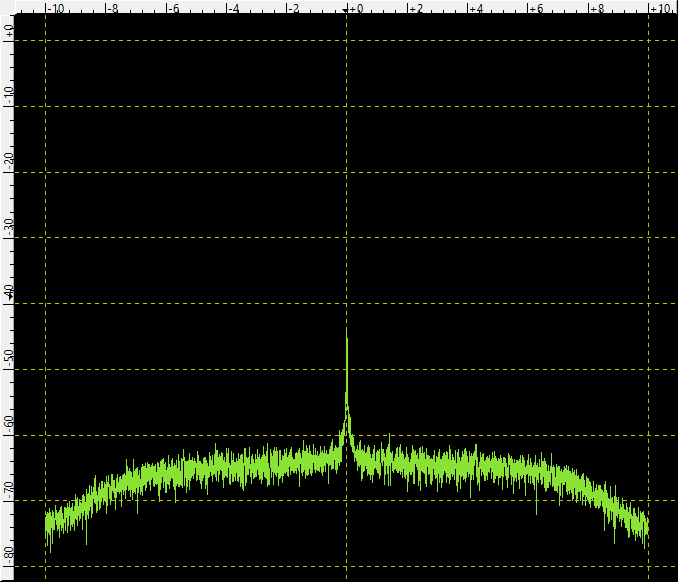
\includegraphics[width=1\linewidth, height=5cm]{fig/bandwidth_15MHz.PNG}
   \caption{}
   \label{fig:bw1} 
\end{subfigure}

\begin{subfigure}[b]{0.45\textwidth}
   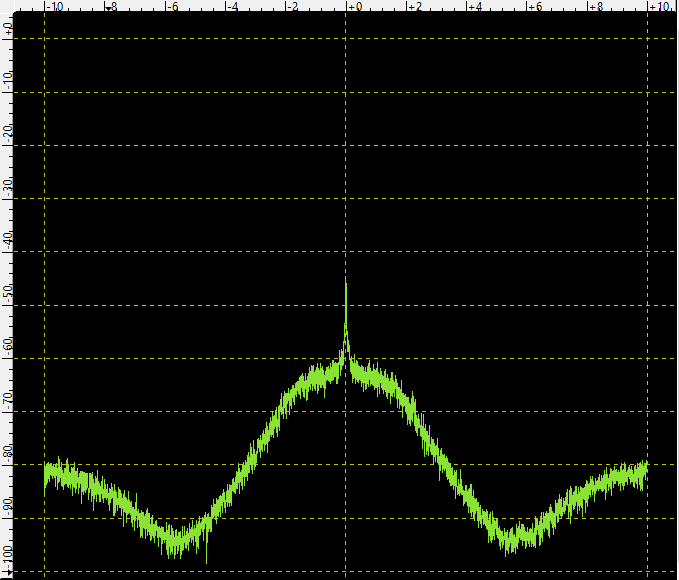
\includegraphics[width=1\linewidth, height=5cm]{fig/bandwidth_3MHz.PNG}
   \caption{}
   \label{fig:bw2}
\end{subfigure}

\caption{ (a) The  frequency spectrum as seen by a receiver with a RX bandwidth of 15 MHz. 
 (b) The  frequency spectrum as seen by a receiver with a RX bandwidth of 3 MHz.  }
\end{figure}


However, figure \ref{fig:bw1} and \ref{fig:bw2} show that a lower bandwidth does not cut a certain outer spectrum away, but rather weakens its gain. 
The set bandwidth of the receiver affects the sent signal as it limits the range of transmitted frequencies. 
Setting the transmitter bandwidth greater than the receiver bandwidth is legal but leads to frequencies that are out of the receiver range.
So in that case only noise at low gain is transmitted.
The local oscillator (center) frequencies of receiver and transmitter might be different from one and another.
In fact, they definetly should be, since close center frequencies of RX and TX leads to echoing which means that the RX chain receives the signal of the transmitter, which directly transmits that same signal of the RX chain. 

\newpage

\begin{figure}[h]
   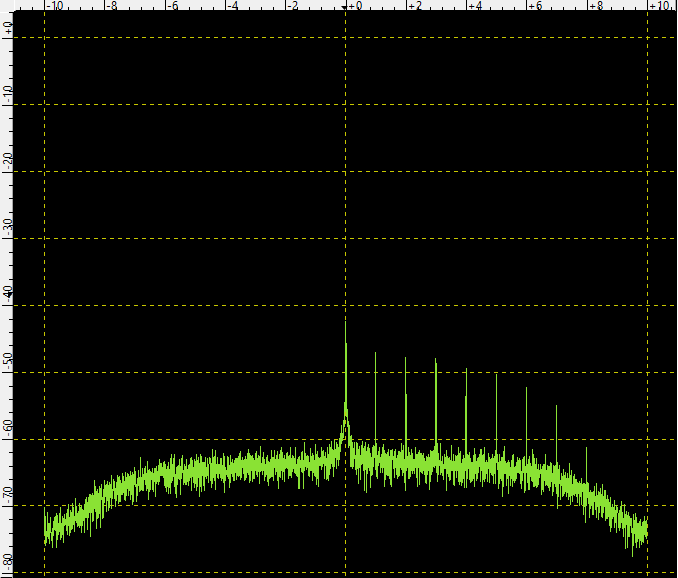
\includegraphics[width=1\linewidth, height=6cm]{fig/echoing.PNG}
   \caption{ The peaks on the right side of the spectrum correspond to the echoing effect when RX LO and TX LO frequencies of the loopback device are close together. }
   \label{fig:echo}
\end{figure}

The right side of the frequency spectrum in figure \ref{fig:echo} shows the echoing effect. 
Having excatly the same center frequencies for both leads to a hold and wind up of the received frequencies, as the received signal is transmitted at the same frequency again.
Echoing also happens when the center frequencies are not exactly the same but in the bandwidth of each other.
The most useful case due to that reasons is when the local oscilator (LO) frequencies are not in each others range.
In that case, a frequency peak received by the loopback device will be re-transmitted at the TX LO plus the relative frequency corresponding to the difference of the RX LO and received frequency peak.

\begin{figure}[h]
   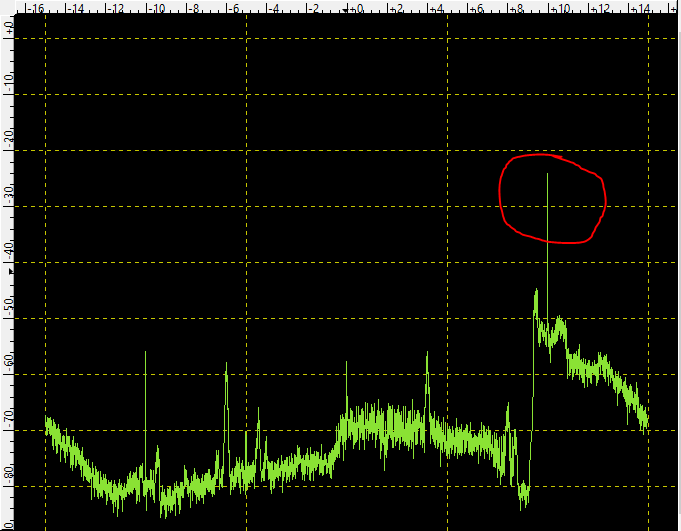
\includegraphics[width=1\linewidth, height=6cm]{fig/example_loopback.PNG}
   \caption{ Received frequency peak at 1210 MHz that was originally transmitted at 1010 MHz and retransmitted using a RX LO of 1000 MHz and TX LO of 1200 MHz for the loopback device. }
   \label{fig:exloop}
\end{figure}

Figure \ref{fig:exloop} shows an example loopback.
The device in loopback mode is setup to RX LO of 1000 MHz and receives a peak at 1010 MHz, so thats a relative frequency of +10 MHz.
The TX LO of the loopback device is 1200 MHz.
The SDR sends the signal at relative +10 MHz, leading to an absolute frequency of 1210 MHz.
The example shows that the transmitted signal (for example, received by an other AdlamPluto) most likely  looks similar to the received signal of the original SDR in loopback mode.




\section{Implementation of detector}
\label{sec:implDetector}
The behavior described in section \ref{sec:behaviourLoopback} is now used to implement a simple detector. The goal is figure out if an AdalmPluto SDR with a specific known loopback local oscillator is in close proximity of another AdalmPluto SDR . 
This is done in two different ways.
The first approach is by only comparing a threshold gain.
The idea is that a specific gain threshold is undercut at a certain distance.
The second one is by calculating the correlation between the received and sent signal.
The idea is to detect the exact moment of signal loss using correlation, then reconstructing the distance using time measurements.


\subsection{Hardware Setup}
\label{subsec:hardware_setup}
The hardware consists of two AdalmPluto with the standard antennas. 
One AdalmPluto is in analog loopback mode and has a RX center frequency of 1000 MHz and a TX center frequency of 1200 MHz.
The sample-rate is 30 MSPS.
The RX bandwidth is 4 MHz.
The TX bandwidth is 2 MHz.

The second AdalmPluto has a TX center frequency of 999 MHz and a RX center frequency of 1200 MHz.
The 999 MHz frequency is chosen due to the center frequency being visible as there will always be a small peak at the center frequency.
Therefore, a 1 MHz signal message is sent at the 999 MHz LO, leading to an absolute frequency peak of 1000 MHz.
Bandwidth and sample rate stay the same for both AdalmPlutos.
The AdalmPluto beeing not in loopback mode collects the samples used for further processing, as described in section \ref{subsec:Software}.



\subsection{Software}
\label{subsec:Software}
Since the loopback mode is a feature of the AdlamPluto and not an external code, it can be activated manually using IIO-oscisloscope, Python or any other suitable software.
When using Python, the attribute "sdr.loopback" is set to 2, which refers to the analog-RX-to-TX loopback mode.
The second AdalmPluto is setup using a Python script in order to gather measurements into a buffer used for detection.
The script generates a  1 MHz signal and transmitts it.
After that, the AdalmPluto collects samples into the buffer.
When the buffer is full, post processing starts.
The two approaches described in \ref{sec:implDetector} can now be applied:
We define to see the signal either if the RX LO exceeds a threshold or the signal correlation is greater than another threshold.
For calculating correlation, a snapshot of the RX frequency spectrum is stored when transmission starts.
This is then correlated with the current frequency spectrum.
Using only the correlation method is more secure, since the amplitude method theoretically leaves the chance of an alternative sender emitting the signal.
The correlation does not use the full received signal but only the parts covered by the transceiver's 2 MHz spectrum. 
For further information please refer to the Python scripts that can be found on github \cite{gitscripts}.
 
\subsection{Experimental Results}
\label{subsec:experimental_results}

\begin{figure}
\centering

\begin{subfigure}[b]{0.45\textwidth}
   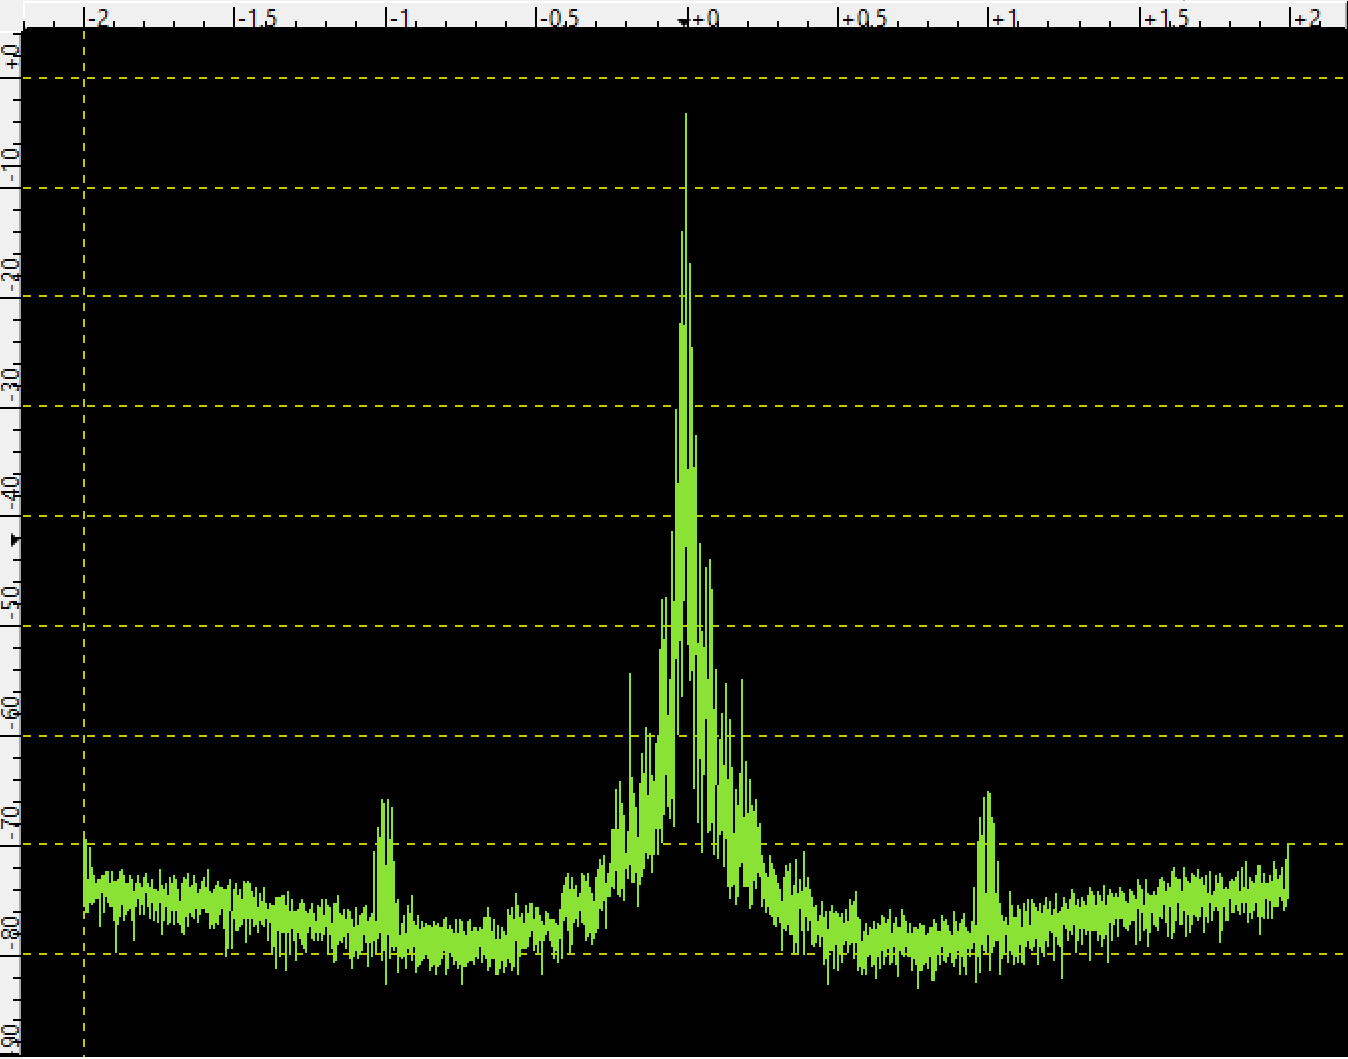
\includegraphics[width=1\linewidth, height=4cm]{fig/loopback_near.PNG}
   \caption{}
   \label{fig:lnear}
\end{subfigure}

\begin{subfigure}[b]{0.45\textwidth}
   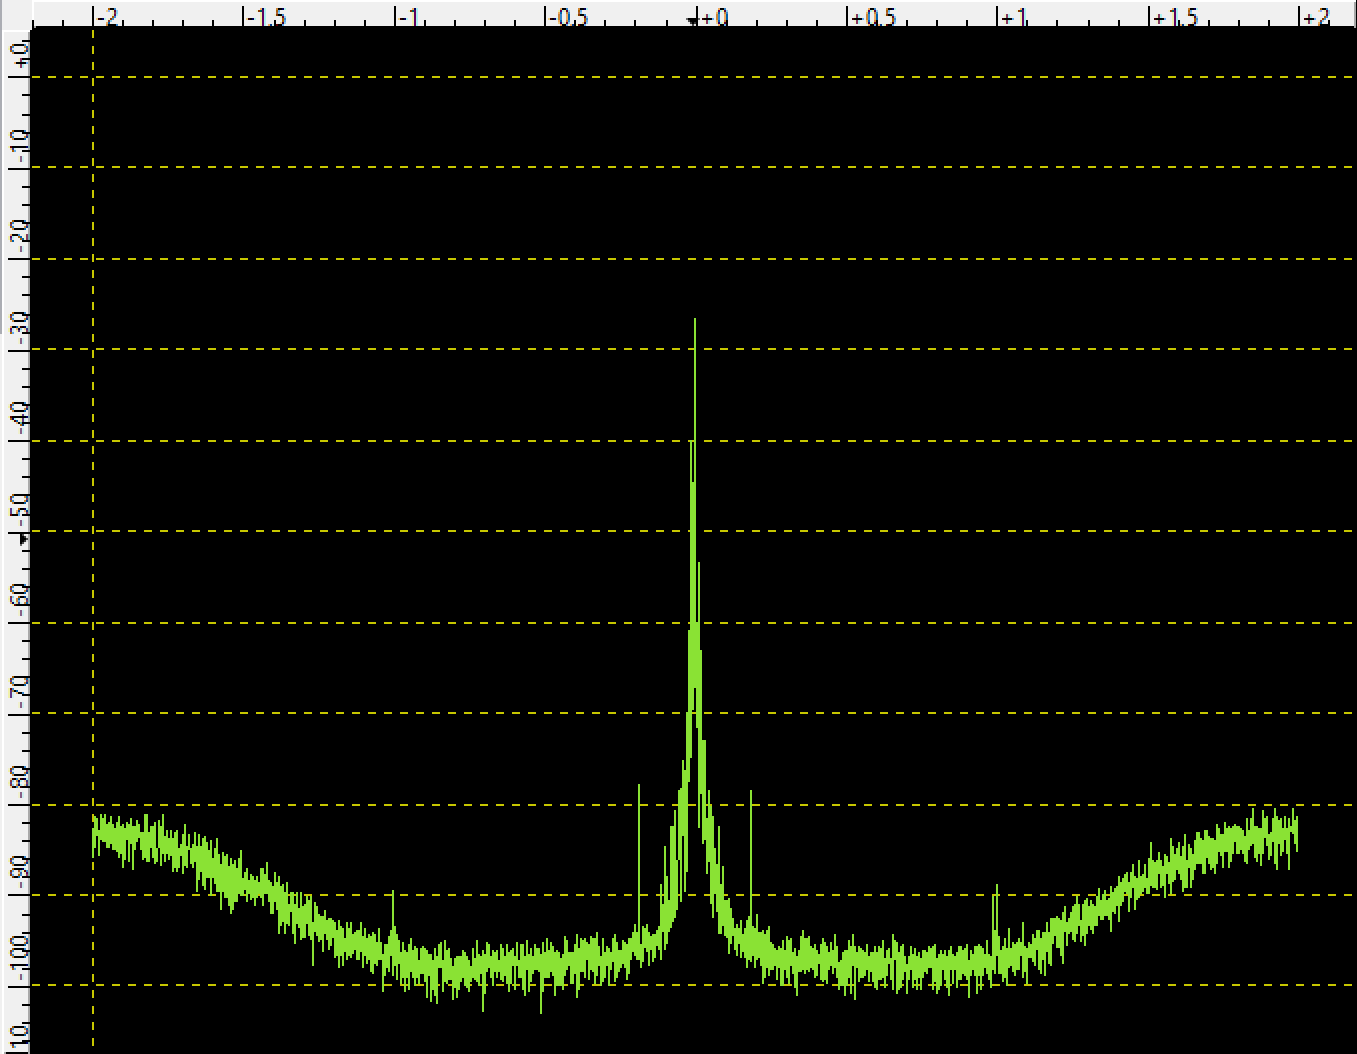
\includegraphics[width=1\linewidth, height=4cm]{fig/loopback_far.PNG}
   \caption{}
   \label{fig:lfar}
\end{subfigure}

\begin{subfigure}[b]{0.45\textwidth}
   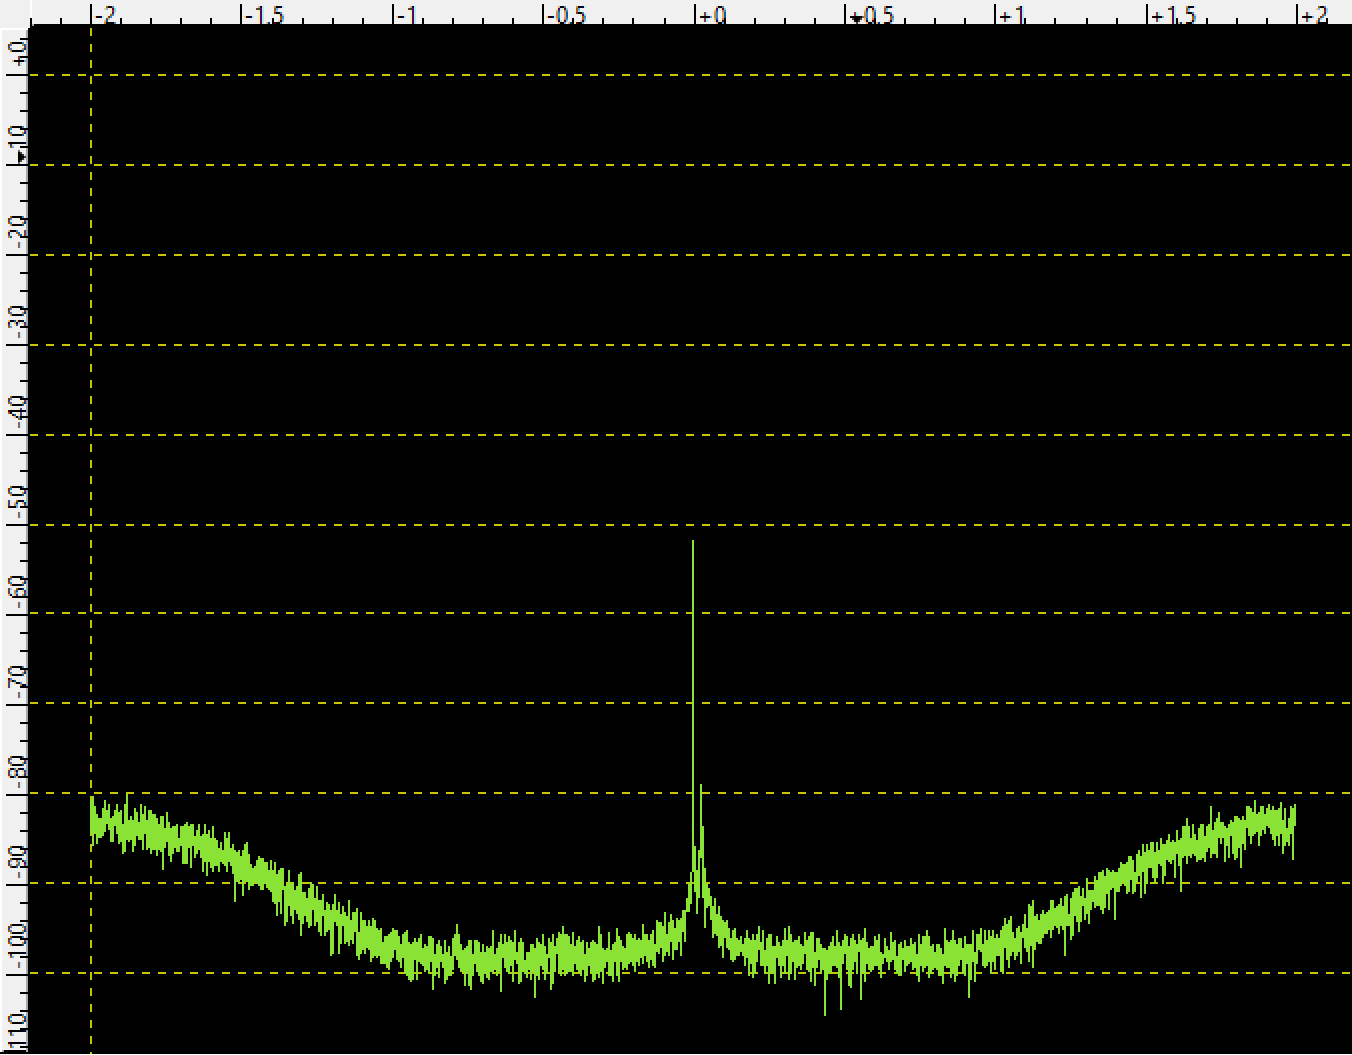
\includegraphics[width=1\linewidth, height=4cm]{fig/loopback_18m_far.PNG}
   \caption{}
   \label{fig:l18far}
\end{subfigure}

\begin{subfigure}[b]{0.45\textwidth}
   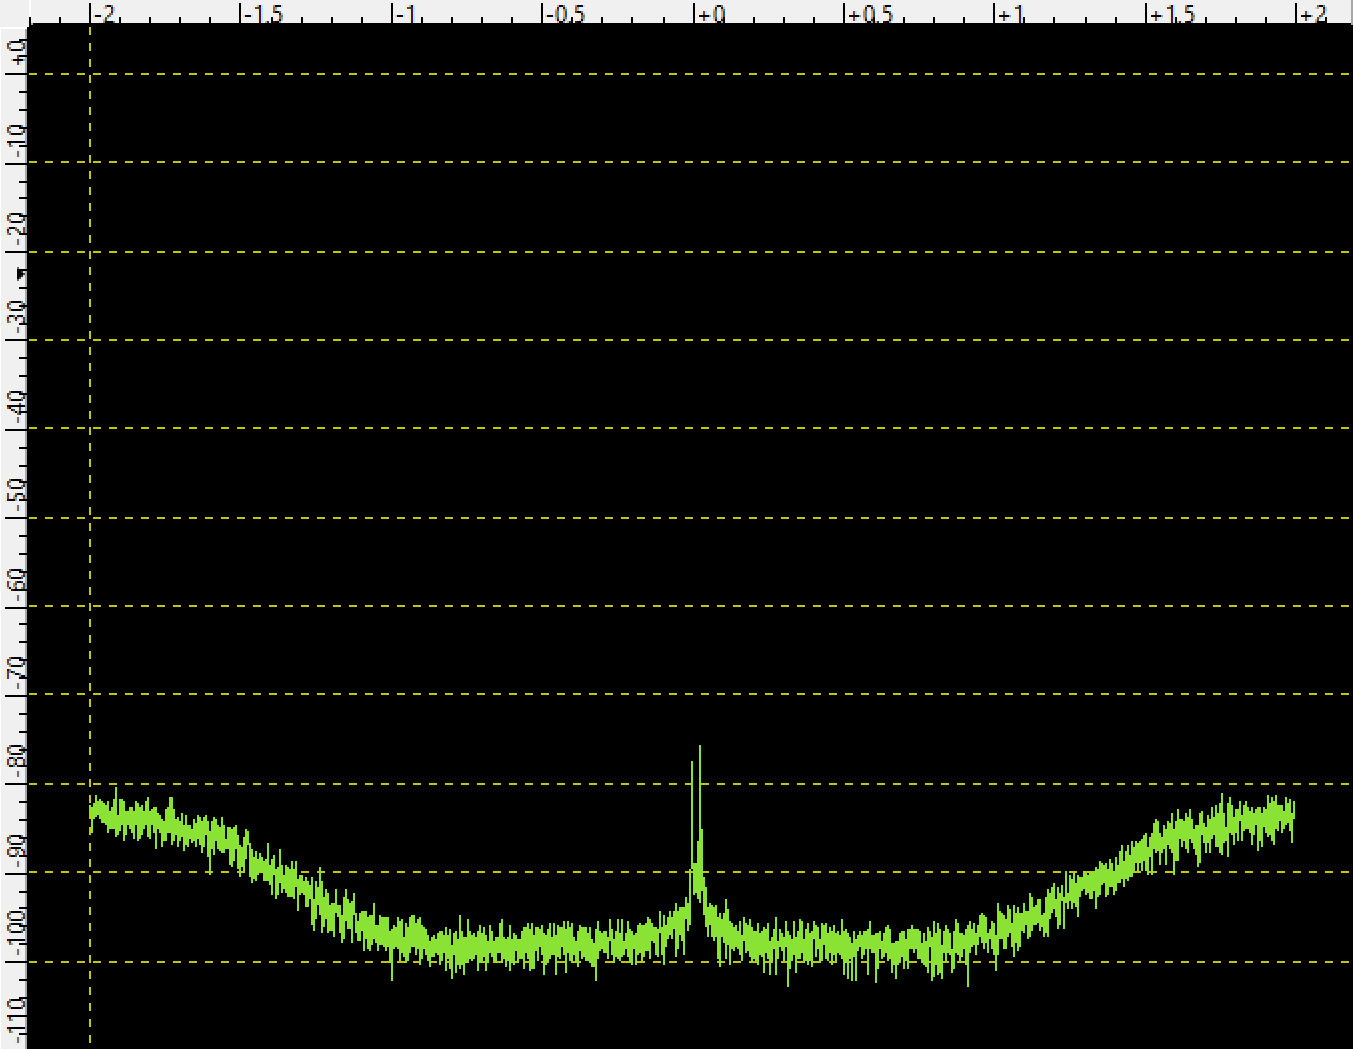
\includegraphics[width=1\linewidth, height=4cm]{fig/loopback_50m_far.PNG}
   \caption{}
   \label{fig:l50far}
\end{subfigure}

\begin{subfigure}[b]{0.45\textwidth}
   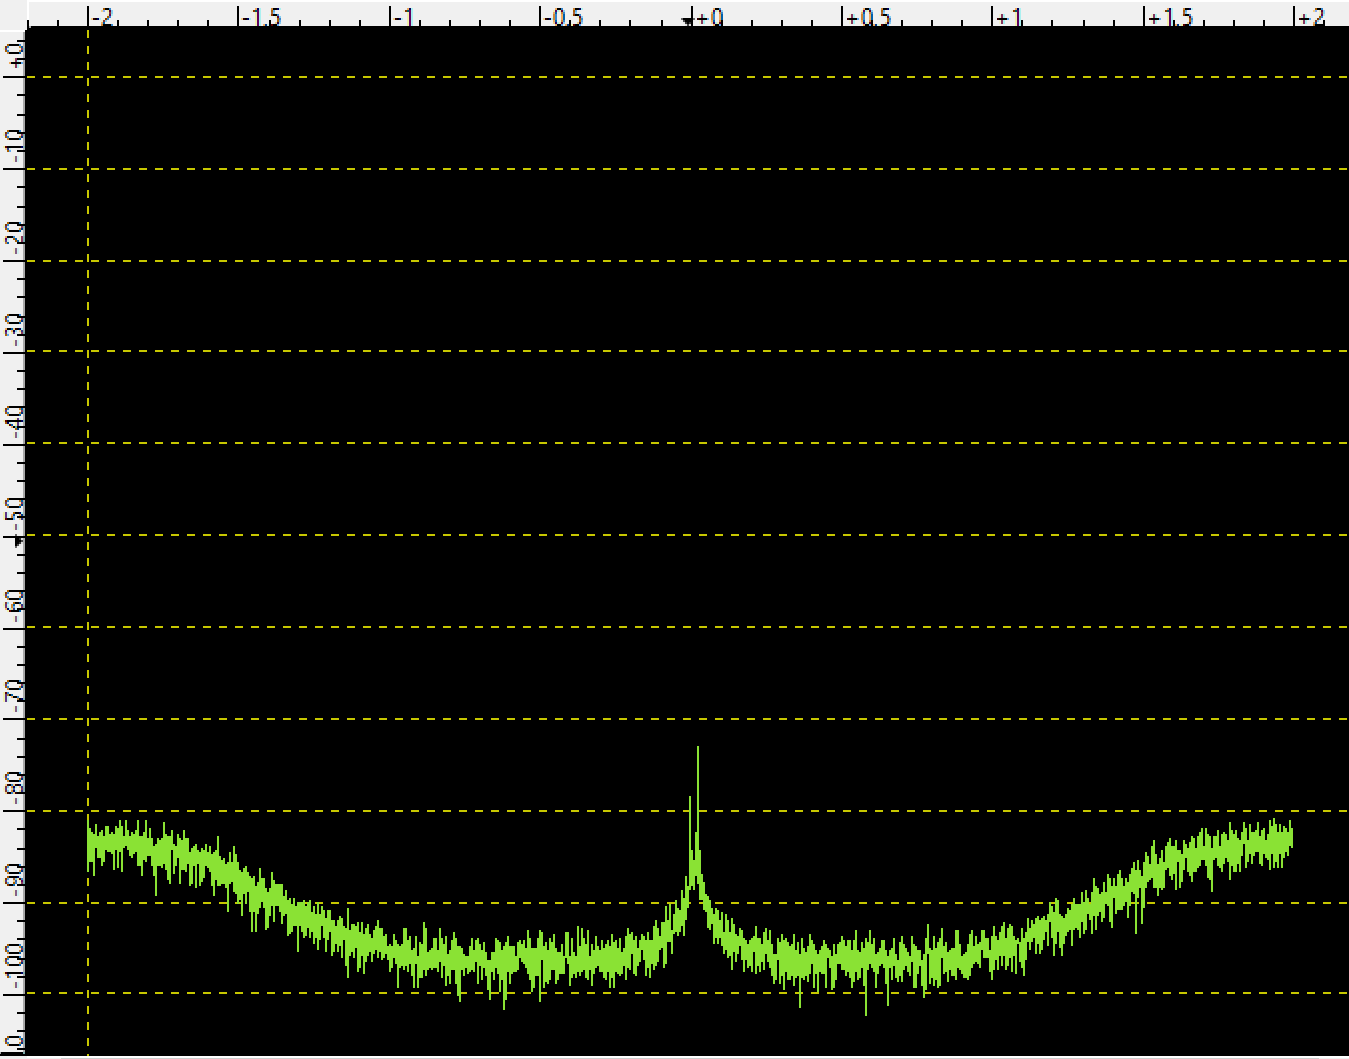
\includegraphics[width=1\linewidth, height=4cm]{fig/loopback_nosignal.PNG}
   \caption{}
   \label{fig:lnosig} 
\end{subfigure}

\caption{ Frequency spectrum at the receiver at (a) 5 cm (b) 1 m (c) 18 m (d) 50 m (e) no signal.  }
\end{figure}

Figure \ref{fig:lnear} to \ref{fig:lnosig} show the transmitted and received signal in different distances as well as the received signal when no signal is transmitted.
As can be seen, a detection of only up to one meter seems feasible for the detection using the amplitude approach. 
Using the correlation method, the other pluto can be detected in a range of about 20 m.
Furthermore, a significant letdown is experienced using the loopback mode:
Sometimes setting up the analog loopback modes resets the other components of the AdlamPluto, which makes it not usable for more than experimental results. Also the loopback mode itself is disabled, without any instruction at all by the user.
However, this was not tested using yet another SDR, so theoretically it could just be due to a bug corresponding to the SDRs used in this report specifically. 


\section{Challenges of range detection with Loopback Mode}
\label{sec:ChallengeDetection}
The next step naturally is trying to detect the exact range between two AdalmPlutos where one of which is operating in loopback mode.

\begin{figure}
   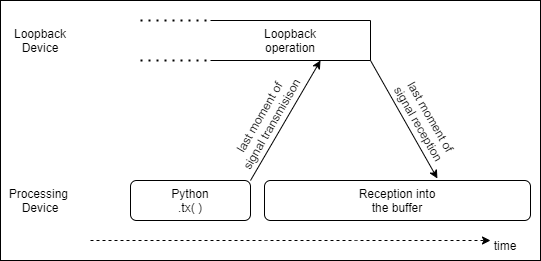
\includegraphics[width=1\linewidth, height=4cm]{fig/periods_block.png}
   \caption{ Simplified block diagram of propagation and processing periods. }
   \label{fig:block}
\end{figure}

Figure \ref{fig:block} is a block diagramm showing the propagation and processing periods.
To determine the exact range between the two SDRs we have to know the full propagation time only. 
The distance could then be calculated using an estimate for the propagation speed (e.g. light speed). 
Therefore, the processing time for the loopback-operation must be known as well as the exact time when the transmission ended and the exact time when the received signal ends.
However, the limitations regarding hardware as well as software addressed in the next section prevent an exact evaluation.

\subsection{Limitations of PlutoSDR and Python}
\label{sec:LimitationPLutoSDR}
There are several problems with exact time measurement.
First of all, when using Python, the .tx( \textit{signal} ) function for writing the buffer to the SDR takes longer than the signal duration.

\begin{figure}[h]
   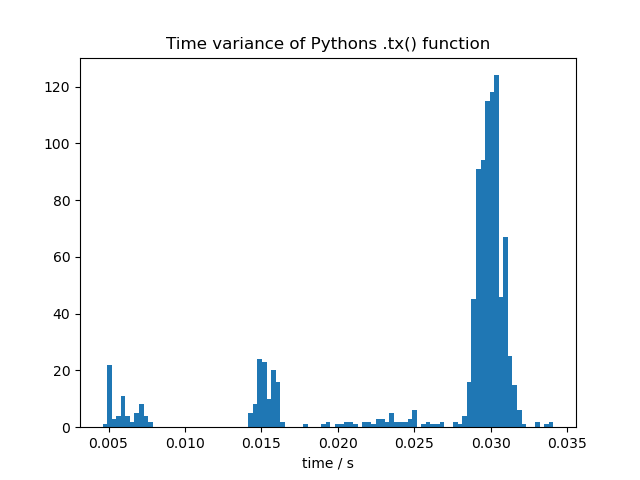
\includegraphics[width=1\linewidth, height=7.5cm]{fig/python_tx_var.png}
   \caption{ Histogram of the sdr.tx( ) function times of the Python API }
   \label{fig:pytimes}
\end{figure}

Furthermore, the function time is not constant for a given signal but rather has a wide variance in duration which can be seen in figure \ref{fig:pytimes}.
Also, its not clear if the transmission starts or ends with that statement (or even something in between).
The time range between the shortest and longest tx()-function is $0.034s-0.005=0.029s$,  correspondents to a travel distance of 8700km,  therefore a detected range difference of 4350km. Even the variance of the data corresponds to a distance variance of approximately 15 km, which makes an exact range measurement impossible, especially when our range of detection is limited by the approximately 50meter, after which no signal is received.
One idea to avoid the dependence on this vague time would be to use such a short signal that when the receiver is started we capture the original transmitted signal first, then nothing, and finally the loopbacked  signal all in one buffer.
There are several problems with this method.
First of all, such a short signal is not enough to generate a noticeable peak at the AdalmPluto.
Secondly, we can only start receiving after transmission ends.
However, this swap from transmit to receive mode is not faster than the time needed for the distance between the two antennas. 
This means that the only way to measure the exact propagation time is to wait until the signal is no longer received, because the buffer that is first written after transmission always holds the re-sent signal already.
Consequently, the only chance to get a useful evaluation is the utilization of hardware-based possibilities for time detection.
Therefore, the buffer can be used for time analysis, as we can use the well defined sampling rate to calculate how much time has passed after a specific number of samples.

\subsection{Passive radar as alternative}
\label{sec:Alternatives}
Even without using the loopback mode, the sending and receiving time uncertainties are too large for an exact distance measurement.
An alternative that overcomes these shortcomings is the passive radar.
Feng et al. \cite{sdrpassive} show how low cost SDR receivers can be used to implement a passive RADAR based on DVB-T signals.
Rooke \cite{plutopassive} shows a native implementation of a passive RADAR running on the AdalmPluto.
The idea is to take an existing signal like DVB-T or radio.
If there is a big reflecting object (car, bicycle), it reflects those signals.
At the receiver side, the signal is then received twice but with different phases.
From this phase difference the corresponding distance can be calculated.
Of course, it is not unambiguous, as a difference of one wavelength leads to the same phase shift.
Also, a distance of exactly the wavelength that's been used is not detectable.
Since the passive radar approach only relies on the received signal and not on any time measurement when this signal is received (or other absolut times) but only on phase difference it is detectable by the AdlamPluto very well despite the limitations.

\subsection{Amplitude approach as alternative}
\label{sec:Alternatives2}
Also not with the necessity of the Loopback-mode, but with the necessity of a second PlutoSDR, is the amplitude approach. The basic idea is to correlate the amplitude of the signal with a distance. The pluto, which would have to be detected, sends a signal at a specific power. Sending with maximum power is not necessarily the best solution, because the receiving Pluto would receive a Signal at zero dB for minimal distances. Therefore a working range has to be defined. Of course, any other Signal at this frequency would lead to false detection. Although we don't focus on the aspect of security by hackers, the possibility of a frequency at that range is given by the environment. Therefore a modulation or code should be sent as confirmation. 
The loopback mode could be used for this approach, as seen in figure \ref{fig:lnear} this would be possible. The pure amplitude approach just by one signal still leaves the possibility for false detection of other signals. Therefore, again a modulation of the signal would be required. 
Therefore the use of Loopback-mode has no advantage over the use of direct communication. Empirical results show that loopback mode does not work well with small amplitudes, meaning that the loopback device receives at a far distance a minimum, but visible signal, but the received signal of the loopback does not show the minimal peak anymore. Therefore an active sending signal would provide a better range.
All these approaches are very sensitive to any sort of disturbance or attenuation of the signal like walls or other obstacles, which are not a big problem for the time measurement approach, as long as a minimal signal is received.
There was no implementation of this approach because this work laid on time measuring approach for radar, which would be better than a pure amplitude approach if it would be realizable. 


\section{Conclusion}
\label{sec:conclusion}
The behavior of the loopback mode was analyzed.
We implemented the detection of an AdalmPluto SDR in loopback mode in two ways.
Any usefull distance measurements are not possible due to the practical limitations of Python and the AdlamPluto.
The passive radar and teh amplitude approach were introduced as working alternatives due to its independence to the described limitations. 




\appendices

\bibliographystyle{bibliography/IEEEtran}

\bibliography{bibliography/IEEEabrv,bibliography/bibliography.bib}

\end{document}


